\documentclass[a4paper,11pt]{article}
\usepackage{amsmath,amsthm,amsfonts,amssymb,amscd,amstext,vmargin,graphics,graphicx,tabularx,multicol} 
\usepackage[francais]{babel}
\usepackage[utf8]{inputenc}  
\usepackage[T1]{fontenc} 
\usepackage{pstricks-add,tikz,tkz-tab,variations}
\usepackage[autolanguage,np]{numprint} 

\setmarginsrb{1.5cm}{0.5cm}{1cm}{0.5cm}{0cm}{0cm}{0cm}{0cm} %Gauche, haut, droite, haut
\newcounter{numexo}
\newcommand{\exo}[1]{\stepcounter{numexo}\noindent{\bf Exercice~\thenumexo} : \marginpar{\hfill /#1}}
\reversemarginpar


\newcounter{enumtabi}
\newcounter{enumtaba}
\newcommand{\q}{\stepcounter{enumtabi} \theenumtabi.  }
\newcommand{\qa}{\stepcounter{enumtaba} (\alph{enumtaba}) }
\newcommand{\initq}{\setcounter{enumtabi}{0}}
\newcommand{\initqa}{\setcounter{enumtaba}{0}}

\newcommand{\be}{\begin{enumerate}}
\newcommand{\ee}{\end{enumerate}}
\newcommand{\bi}{\begin{itemize}}
\newcommand{\ei}{\end{itemize}}
\newcommand{\bp}{\begin{pspicture*}}
\newcommand{\ep}{\end{pspicture*}}
\newcommand{\bt}{\begin{tabular}}
\newcommand{\et}{\end{tabular}}
\renewcommand{\tabularxcolumn}[1]{>{\centering}m{#1}} %(colonne m{} centrée, au lieu de p par défault) 
\newcommand{\tnl}{\tabularnewline}

\newcommand{\bmul}[1]{\begin{multicols}{#1}}
\newcommand{\emul}{\end{multicols}}

\newcommand{\trait}{\noindent \rule{\linewidth}{0.2mm}}
\newcommand{\hs}[1]{\hspace{#1}}
\newcommand{\vs}[1]{\vspace{#1}}

\newcommand{\N}{\mathbb{N}}
\newcommand{\Z}{\mathbb{Z}}
\newcommand{\R}{\mathbb{R}}
\newcommand{\C}{\mathbb{C}}
\newcommand{\Dcal}{\mathcal{D}}
\newcommand{\Ccal}{\mathcal{C}}
\newcommand{\mc}{\mathcal}

\newcommand{\vect}[1]{\overrightarrow{#1}}
\newcommand{\ds}{\displaystyle}
\newcommand{\eq}{\quad \Leftrightarrow \quad}
\newcommand{\vecti}{\vec{\imath}}
\newcommand{\vectj}{\vec{\jmath}}
\newcommand{\Oij}{(O;\vec{\imath}, \vec{\jmath})}
\newcommand{\OIJ}{(O;I,J)}


\newcommand{\reponse}[1][1]{%
\multido{}{#1}{\makebox[\linewidth]{\rule[0pt]{0pt}{20pt}\dotfill}
}}

\newcommand{\titre}[5] 
% #1: titre #2: haut gauche #3: bas gauche #4: haut droite #5: bas droite
{
\noindent #2 \hfill #4 \\
#3 \hfill #5

\vspace{-1.6cm}

\begin{center}\rule{6cm}{0.5mm}\end{center}
\vspace{0.2cm}
\begin{center}{\large{\textbf{#1}}}\end{center}
\begin{center}\rule{6cm}{0.5mm}\end{center}
}



\begin{document}
\pagestyle{empty}
\titre{Interrogation: Grandeurs et périmètres }{Nom :}{Prénom :}{Classe}{Date}

\vspace*{0.5cm}

\begin{flushleft}
\begin{tabular}{|m{6cm}|m{2.5cm}|m{2.5cm}|m{2.5cm}|m{2.5cm}|}
\hline 
\textbf{Compétences} & \begin{center}
\textbf{Très bonne maîtrise}
\end{center} & \begin{center}
\textbf{Maîtrise satisfaisante}
\end{center}  & \begin{center}
\textbf{Maîtrise faible}
\end{center} & \begin{center}
\textbf{Maîtrise insuffisante}
\end{center} \\ 
\hline 
Je dois connaître et savoir convertir les unités de longueur ou de masse &  &  & &\\
\hline
Je dois savoir calculer le périmètre d'un polygone &  &  & & \\ 
\hline
Je dois connaître la formule donnant le périmètre d'un cercle &  &  &  &\\ 
\hline 
Je dois savoir calculer le périmètre d'une figure composée  &  &  &  &\\ 
\hline 


\end{tabular} 
\end{flushleft}

\vspace*{0.5cm}



\exo{3} Cours :\\

 Compléter les égalités suivantes :\\

\bmul{3}

\qa 0,021 km = ............... dam\\

\qa 2 501 mm = ............... dm\\

\columnbreak

\qa 0,53 dam = ............... cm \\

\qa 164 cg = ............... g\\

\columnbreak

\qa 4,5 t = ............... kg\\

\qa 423 mg = ............... cg\\

\emul

\vspace*{0.5cm}

\exo{2} En sachant que le côté d'un carreau mesure 1 cm. Déterminer le périmètre de chaque figure.

\bmul{2}

\includegraphics[scale=0.7]{carreauperimetre.eps} 

\columnbreak

\vspace*{1cm}

\bmul{2}

$P_{fig3}= . . . . .  . $\\

$P_{fig7}= . . . . .  . $\\

\columnbreak

$P_{fig4}= . . . . .  . $\\

$P_{fig8}= . . . . .  . $\\

\emul


\emul

\vspace*{0.5cm}

\exo{3} Calculs de périmètres\\

\initq \q Calculer le périmètre d'un carré de côté 3,2 cm.\\
\reponse[3]\\

\newpage


\vspace*{0.5cm}

\q Calculer le périmètre d'un rectangle de longueur 8 cm et de largeur 5,5 cm.\\
\reponse[3]\\

\q Calculer la circonférence d'un cercle de 3,5 m de rayon.\\
\reponse[4]\\

\vspace*{0.5cm}

\exo{2} Calculer le périmètre de la figure suivante.\\
\bmul{2}


\includegraphics[scale=0.5]{perimetre.eps} 


\columnbreak

\noindent \reponse[7]\\

\emul

\exo{} Bonus

\bmul{2}

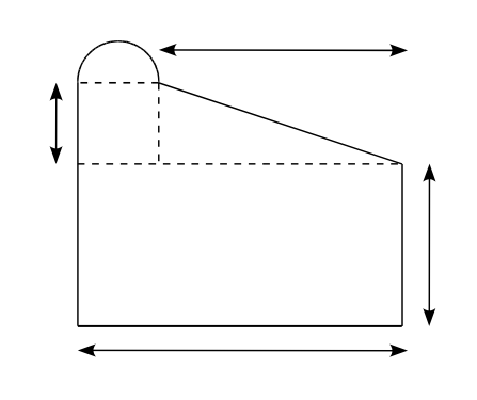
\includegraphics[scale=0.9]{bonus.eps} 

\columnbreak

\vspace*{0.5cm}

Ce dessin représente le plan de la façade d'une maison.\\

\initq \q Compléter ce plan en y ajoutant les dimensions réelles sachant que 1 cm   sur   le   plan représente 2,5 m dans la réalité.\\

\emul

\q Calcule le périmètre de la façade de cette maison au décimètre carré près.\\
\reponse[6]

\end{document}
